% !TEX encoding = UTF-8
% !TEX TS-program = pdflatex
% !TEX root = ../tesi.tex

%**************************************************************
\chapter{Analisi comparativa dei protocolli REST e GraphQL}
\label{cap:analisi-comparativa}
%**************************************************************
\intro{In questo capitolo verrà svolta l'analisi comparativa tra i due protocolli REST e GraphQL, sia dal punto di vista teorico che da quello pratico .}\\
%**************************************************************
%\section{Analisi comparativa teorica}
%\label{sec:analisi-comparativa-teorica}
%Per analisi comparativa teoria s'intende tutti quegli aspetti che differenziano i due protocolli GraphQL e REST
\section{Introduzione}
REST è stato ed è tutt'oggi lo standard più seguito per la realizzazione delle Web API, tuttavia dopo l'uscita di GraphQL gli sviluppatori hanno iniziato ad utilizzare sempre di più la nuova tecnologia. Infatti GraphQL ha portato con se delle interessanti soluzioni per molti dei problemi e dei vincoli dello stile architetturale REST.\\
L'innovazione portata da GraphQL è stata apprezzata in larga scala tra gli sviluppatori, a conferma di ciò è possibile visualizzare nell'immagine \ref{graphQL-usage-chart} l'aumento nell'utilizzo di questa tecnologia con il passare degli anni.
\FloatBarrier
\begin{figure}[!ht]
\centering
\includegraphics[width=1\linewidth]{immagini/GraphQLUsageChart.png}
\caption{Grafico sull'utilizzo di GraphQL negli anni.}
\label{graphQL-usage-chart}
\end{figure}
\FloatBarrier
Nel seguente capitolo verranno analizzati nel dettaglio e paragonati i due protocolli, sotto tutti i punti di vista, mettendo in risalto vantaggi e svantaggi di ciascuno; infine verranno riportate le deduzioni elaborate durante lo stage sul protocollo che è meglio seguire in base all'applicativo che si vuole sviluppare.
\section{Analisi comparativa}
Come sottolineato in precedenza, GraphQL e REST hanno diversi aspetti che li differenziano. La più grande differenza tra questi due protocolli è legata alla loro natura: infatti quando si fa riferimento a REST, si sta parlando di uno stile architetturale, dunque di un modo di costruire le proprie API le quali, se rispettano i vincoli REST illustrati al punto \ref{principi-REST}, vengono definite RESTful. Quando si fa riferimento a GraphQL invece, si sta parlando di un linguaggio di query fortemente tipizzato.\\\\
Di seguito è presente un'analisi comparativa dettagliata per ciascun aspetto che differenzia i due protocolli di data fetching.
\subsection{Endpoints}
La prima grossa differenza tra i due protocolli riguarda gli endpoint. Per endpoint si intendono i punti di accesso forniti dal server per permettere al client di eseguire richieste.\\
Lo stile REST prevede l'utilizzo di più endpoint, sfrutta infatti la molteplicità degli endpoint per differenziare le richieste possibili. Quando un client implementa una richiesta a delle REST API deve sapere esattamente a quale endpoint inviare la richiesta per ricevere i dati necessari. In figura \ref{REST-endpoints} viene rappresentato la struttura degli endpoint multipli di un REST server con il client che invia diverse richieste ai diversi endpoint.
\FloatBarrier
\begin{figure}[!ht]
\centering
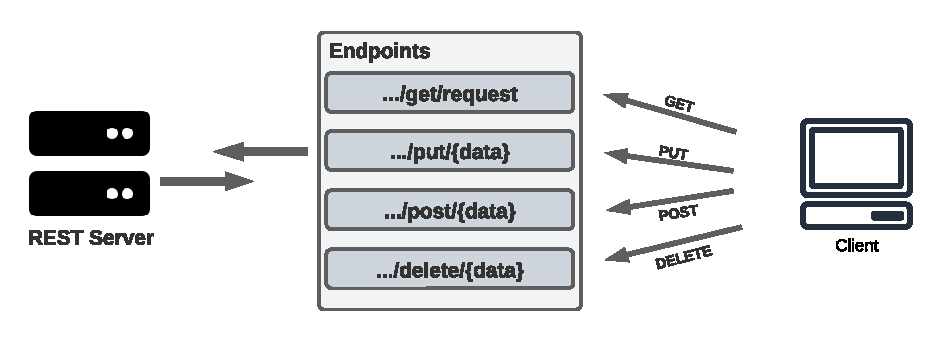
\includegraphics[width=1\linewidth]{immagini/RESTEndpoints.pdf}
\caption{Gli endpoints multipli in REST.}
\label{REST-endpoints}
\end{figure}
\FloatBarrier
Con GraphQL questo non avviene, infatti GraphQL prevede l'esposizione di un unico endpoint. A questo singolo endpoint possono essere inviate tutte le richieste inserendo nel body della richiesta la query, la mutation o la subscription. In figura \ref{GraphQL-endpoint} è possibile visualizzare come il GraphQL server fornisca un unico endpoint e come il client invii tutti i tipi di richieste allo stesso medesimo endpoint.
\FloatBarrier
\begin{figure}[!ht]
\centering
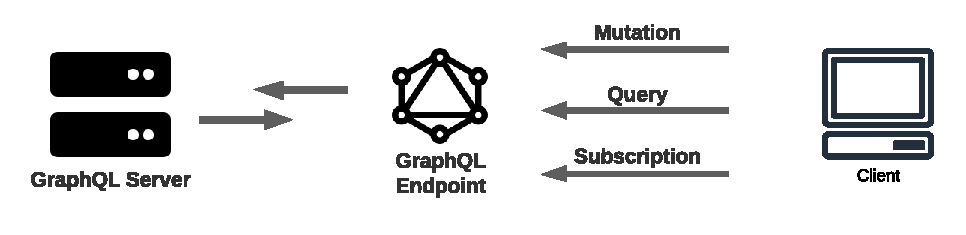
\includegraphics[width=1\linewidth]{immagini/GraphQLEndpoint.pdf}
\caption{Il singolo endpoint GraphQL.}
\label{GraphQL-endpoint}
\end{figure}
\FloatBarrier
A proposito di ciò viene riportata di seguito una citazione di Lee Byron, il co-creatore di GraphQL:
\begin{quoting}
  \textit{"Think in graphs, not endpoints."}
\end{quoting}
Con questa fra L. Byron rappresenta perfettamente l'idendità di GraphQL che si propone come sistema innovativo che prevede di distribuire le risorse ordinatamente su un grafo e non, come in REST, su diversi endpoint.
\subsection{Overfetching e Underfetching}
La questione dell'overfetching e underfetching è uno degli aspetti che viene maggiormente considerato nella decisione architetturale riguardo quale protocollo di data fetching utilizzare tra REST e GraphQL.\\
Lo stile architetturale REST non prevede di definire lato client esattamente quali dati ricevere. Un client che necessita un certo insieme da un server con REST API, è costretto ad eseguire una o più richieste e dunque a prendersi in carico della rielaborazione dei dati. Per uno sviluppatore backend è molto complesso riuscire a creare delle REST API che siano in grado di soddisfare esattamente le tutte le richieste dei client.
L'introduzione di GraphQL come nuovo protocollo di data fetching ha posto una soluzione a questo problema, permettendo al client di specificare esattamente la forma e il quantitativo di dati necessari. Quando si decide di implementare un applicativo e si valuta quale protocollo di data fetching utilizzare, questo è sicuramente un punto da considerare.\\
\paragraph{Overfetching}
Quando si parla di overfetching si fa riferimento al fatto che vengano forniti più dati di quanti realmente necessari. Riprendendo come esempio il prototipo visto nel capitolo \ref{casi-uso}, si suppone che il client necessiti della lista degli impiegati e che, per ciascun impiegato, necessiti  esclusivamente l'id e il nome. Qualora si tratti della version REST del server, il client inviare la richiesta HTTP all'endpoint mappato sul metodo \textit{allEmployee()}, il quale ritorna una lista di impiegati e, per ciascun impiegato, tutti i campi. Di seguito il JSON di risposta che il client riceve in seguito alla richiesta nel caso in cui fossero presenti solo due impiegati:
\begin{verbatim}
  [
    {
        "id": "3AFASDF12F",
        "name": "Matteo",
        "surname": "Verdi",
        "salary": 1500,
        "birth": "1995-02-21"
    },
    {
        "id": "GA14PL3FAV",
        "name": "Marco",
        "surname": "Blu",
        "salary": 1500,
        "birth": "1993-12-20"
    }
  ]
\end{verbatim}
Si può subito notare come i campi \textit{surname}, \textit{salary} e \textit{birth} non siano necessari in quanto il client utilizza solo i campi \textit{id} e \textit{name}. Nel caso del prototipo si tratta di un problema irrisorio data la ridotta grandezza dei dati, tuttavia in applicativi a larga scala che richiedono grossi quantitativi di dati complessi può risultare un problema in termini di occupazione di rete e di rallentamenti dell'applicativo. Questo problema può essere risolto in un server con REST API fornendo endpoint specifici per ciascun tipo di richiesta, tuttavia questa soluzione rischia di introdurre confusione e nel tempo la manutenzione potrebbe risultare sempre più complessa.\\
GraphQL risolve questo problema attribuendo al client la responsabilità di definire quali siano i campi di cui necessita. Questo è possibile specificando nella query i campi richiesti, di seguito l'esempio dell'invocazione contenente a sinistra la query \textit{allEmployees}, mentre a destra il JSON ricevuto in risposta:
\begin{verbatim}
    QUERY                                     JSON RETURNED

    query {                              "data": {
      allEmployees {                        "allEmployees": [
          id                                  {
          name                                   "id": "3AFASDF12F",
          }                                      "name": "Matteo"
        }                                     },
      }                                       {
                                                 "id": "GA14PL3FAV",
                                                 "name": "Marco"
                                              }
                                            ]
                                          }
\end{verbatim}
In GraphQL questo approcio permette di non sovraccaricare inutilmente la rete e di mantenere ordinato e di facile manutenzione la struttura API del server. Lato client è richiesto un maggior sforzo nella specifica della query, ma d'altra parte si evitano problemi di rallentamento o errori dovuti al fetching di grossi quantitativi di dati inutili.
\paragraph{Underfetching}
L'underfetching è il problema opposo all'overfetching, ovvero ciò accade quando il client dopo una richiesta alle REST API riceve solo una parte dei dati necessari. Questo implica che il client deve eseguire più chiamate per ottenere i dati completi.\\
Riprendendo l'esempio precedente nel paragrafo riguardante l'overfetching, qualora il client desiderasse visualizzare i progetti ai quali sta lavorando un impiegato, dovrà prima ricevere la lista degli impiegati e, solo successivamente, ricercare i progetti con l'id dell'impiegato.\\
La stessa medesima operazione utilizzando GraphQL è risolvibile in una sola richiesta:
\begin{verbatim}
  QUERY                                 JSON RETURNED

  query {                           "data": {
    allEmployees {                     "allEmployees": [
      id                                 {
      projects {                           "id": "3AFASDF12F",
          id                               "projects": [
          name                               {
        }                                       "id": "7NFAISH280",
      }                                         "name": "Progetto Beta"
    }                                        },
  }                                          {
                                                "id": "N2A8F234SD",
                                                "name": "Progetto Teta"
                                            }
                                           ]
                                          }
                                        ]
                                      }
\end{verbatim}
A sinistra è possibile visualizzare la query \textit{allEmployees} nella quale viene specificato l'id di ciascun impiegato ed il campo \textit{projects}, il quale, a sua volta, ha specificato i campi \textit{id} e \textit{name}. A destra invece è visualizzato il JSON ritornato con l'impiegato e i due progetti ai quali sta partecipando.
\subsubsection{Utilizzo del protocollo HTTP}
Nonostante entrambi i protocolli non richiedano per forza il protocollo HTTP per funzionare, entrambi nella maggior parte dei casi vengono utilizzati con esso. Per questo motivo viene eseguita un'analisi su come REST e GraphQL si comportano con il protocollo HTTP. \\
I due protocolli comparati utilizzano il protocollo HTTP in maniera molto differente. Lo stile REST alla sua creazione è stato fortemente basato sul protocollo HTTP, per questo motivo lo sfrutta ampiamente. GraphQL invece, per il modo in cui opera, sfrutta solo in parte ed in maniera "stupida" il protocollo HTTP e per questo motivo GraphQL viene spesso definito agnostico rispetto al protocollo di trasporto.
\paragraph{Metodi HTTP}
Per metodi HTTP s'intendono le possibili operazioni che il protocollo HTTP prevede nella comunicazione tra due moduli di rete. Le API REST supportano i metodi POST, GET, PUT e DELETE per la gestione delle risorse sul server e nel caso della POST e della PUT è possibile specificare i dati all'interno del body della richiesta HTTP. GraphQL invece sfrutta solamente l'operazione POST e specifica nel body la query, la mutation o la subscription desiderata.
\paragraph{Codici di stato}
I codici di stato vengono utilizzati per dare informazioni sull'esito di una richiesta HTTP e risultano fondamentali nella comprensione degli errori. Mentre REST utilizza ampiamente i codici di stato nelle risposte, GraphQL ritorna esclusivamente il codice di stato 200 e specifica il problema nel JSON ritornato; talvolta in alcuni GraphQL server, qualora si dovessero verificare degli errori, può essere ritornato anche il codice di stato 500 riferito all'\textit{Internal Server Error}.
\paragraph{Caching}
Per caching s'intende il meccanismo attraverso il quale il browser, il client, i server proxy o altri moduli della rete riescono ad archiviare localmente i dati a cui si accede frequentemente senza dover ogni volta mandare la medesima richiesta al server. Si tratta di fattore importante poiché, se utilizzato correttamente, permette di ridurre il traffico dati tra i moduli della rete e i tempi di latenza, i dati sono recuperabili molto più velocemente e questo è fondamentale per fornire velocemente i dati nei siti web, vengono eseguiti meno accessi al database lato server e le performance di conseguenza migliorano.\\
Il caching è parte integrante del protocollo HTTP e viene ampiamente sfruttato in REST, infatti per il metodo GET e in parte anche per i metodi PUT e DELETE il caching, a meno di direttive specifiche, viene utilizzato di default. Per quanto riguarda il metodo POST il caching non viene utilizzato di default, ma con apposite direttive nell'header della risposta HTTP è possibile permetterlo.\\
Per il modo in cui opera GraphQL, il caching previsto dal protocollo HTTP non viene sfruttato. Per questo motivo, anche nella documentazione GraphQL, viene specificato come sia un dovere del client quello di abilitare e gestire il caching. Alcune librerie permettono di risolvere questo problema, ad esempio il modulo \textit{Apollo} utilizzato per la realizzazione del frontend del prototipo e nella migrazione dell'applicativo SushiLab, include una implementazione del caching di default chiamata \textit{InMemoryCache}.
\subsubsection{Altri aspetti comparativi}
Sono presenti molti altri aspetti che differenziano i due protocolli analizzati. Di seguito vengono riporatati i più importanti.
\paragraph{Documentazione}
La documentazione delle API risulta fondamentale quando uno sviluppatore client necessita di utilizzare i servizi web resi disponibili da un server.\\
Uno degli aspetti più interessanti di GraphQL è proprio quello che si autodocumenta durante la definizione del GraphQL Schema. Infatti definendo il GraphQL schema vengono dichiarati i tipi e la loro struttura campo per campo, le loro relazioni, le query, le mutation, le subscription ed eventuali altri tipi particolari come tipi unione ed enumerazioni. Inoltre il linguaggio SLD, utilizzato nella realizzazione dello schema GraphQL, supporta anche il linguaggio di markup \textit{Markdown} e dunque è possibile, direttamente dal GraphQL schema, specificare ulteriori informazioni su determinati elementi dello schema inserendo delle frasi.\\
Lo sviluppatore client che desidera la documentazione su un determinato schema GraphQL, può facilmente recuperarla con un processo chiamato \textit{Introspection} per il quale è possibile effettuare una query sempre disponibile richiedendo il campo \textit{\_\_schema} e definendo ciò che vuole visualizzare dei tipi nello schema, così facendo può ottenere come risposta direttamente tutte le informazioni che più desidera. Ci sono inoltre dei tool che permettono di semplificare il processo di instrospezione, ad esempio usando il GraphQL playground.\\
In REST non è previsto nessun modo per documentare le API se non affidandosi a servizi esterni, come ad esempio il noto toolset opensource \textit{Swagger}.
\paragraph{Sicurezza}
Si tratta di un fattore fondamentale per la trasmissione sicura di dati tra moduli sulla rete. Le REST API supportano i protocolli crittografici, ad esempio il Transfer Layer Security il quale assicura che i dati che vengono passati tra moduli della rete rimangano invariati e privati. Inoltre sono presenti moltpelici specifiche per garantire la sicurezza nello scambio di messaggi attraverso API REST, tra le quali: JWT, JWS, JWk, ecc...\\
Anche GraphQL ha dei modi per l'autenticazione e l'autorizzazione le richieste del client, tuttavia risultano sicuramente meno sviluppati e consolidate rispetto a quelli disponibili con le REST API.\\
Un altro punto critico di GraphQL legato alla sua flessibilità, ovvero al fatto che permetta di richiedere qualsiasi tipo di dato in qualsiasi forma, è quello che proprio per questa ragione sia possibile, se non vengono strutturate bene le risorse, essere vittime di attacchi DoS attraverso query annidate che vanno a sovraccaricare il database e il server. Questa parziale mancanza di GraphQL è dovuta probabilmente al fatto che si tratti di una tecnologia giovane, ma sono presenti sempre più modi per gestire la sicurezza ed evitare questo tipo di situazioni.
\paragraph{Formato dati supportati}
Le REST API supportano diversi tipi di dati come: JSON, XML e YAML. GraphQL dall'altra parte supporta solo il formato JSON.
\paragraph{Versionamento ed evoluzione delle API}
Il versionamento e l'evoluzione delle API sono argomenti molto dibattuti, ci sono diversi filoni di pensiero e diversi approci classici, alcuni prediligono l'evoluzione delle API, altri ritengono necessario versionarle.\\
GraphQL predilige un approcio di evoluzione delle API, infatti è possibile evolvere le proprie GraphQL API introducendo nuovi campi nei tipi e preservando i vecchi campi così da mantenere la retrocompatibilità. A conferma di quanto appena affermato, di seguito viene riportato quanto scritto nella pagina riguardante le migliori pratiche nella documentazione GraphQL:
\begin{quoting}
  \textit{"While there’s nothing that prevents a GraphQL service from being versioned just like any other REST API, GraphQL takes a strong opinion on avoiding versioning by providing the tools for the continuous evolution of a GraphQL schema."}
\end{quoting}
Questo approcio inoltre può essere utilizzato anche con API REST.\\
Per quanto riguarda però l'eliminazione di alcune funzionalità o campi dati, in GraphQL è possibile definire dei campi deprecati con apposite direttive e, quando gli sviluppatori frontend interrogano lo schema con l'introspezione, vengono scoraggiati dall'utilizzare quella determinata funzionalità o campo dati che verrà presto rimossa. A differenza degli schemi di versionamento come il \textit{Semantic Versioning}, in GraphQL non è possibile specificare quando verrà rimosso effettivamente il campo deprecato. Anche con le REST API può essere indicato un campo deprecato, ma questo è possibile specificarlo solo nella documentazione delle API.\\
Dunque in accordo con quanto riportato precedentemente dalla documentazione GraphQL, nulla impedisce il versionamento in GraphQL, per questo sono stati ideati dei modi per versionare anche le GraphQL API, come ad esempio includere nei vari tipi dei campi versionamento e dunque in base alla versione trattare i vari campi in maniere differenti. In REST invece il versionamento avviene in maniera differente, infatti vengono utilizzati principalmente due approci, uno che prevede di realizzare più versioni di API e richiede però che venga specificato la versione nell'URI della chiamata; l'altro che invece richiede di specificare la versione includendola nell'header della richiesta HTTP.
\paragraph{Trasmissione di dati in tempo reale}
Nelle Real Time Application è necessario ricevere i dati dal server in tempo reale. Questo non è possibile se il server fornisce delle REST API, a meno che non vengano utilizzati degli escamotage come ad esempio il \textit{long pooling} secondo il quale il server, dopo aver ricevuto una richiesta dal client, mantiene aperta la connessione fino a che non arrivano dati in tempo reale e quel punto invia la risposta al client, il quale subito dopo invia una nuova richiesta al server per riaprire immediatamente la connessione.\\
In GraphQL non serve utilizzare degli escamotage per permettere questo tipo di scambio dati in tempo reale, infatti è stato reso disponibile un tipo detto \textit{Subscription}, spiegato precedentemente nel capitolo \ref{casi-uso}, che permette al client di "iscriversi" ad un certo tipo di dati e, al verificarsi di un certo evento, il server invia direttamente i dati al client senza che il client li richieda. Il tutto è implementato con i WebSocket che permettono di mantenere la connessione server-client attraverso una connessione TCP. \\
È possibile utilizzare in WebSocket anche con API REST, ma risulta essere comunque un adattamento guidato dall'esigenza di poter utilizzare connessioni bidirezionali, non si tratta di una funzionalità prevista nella natura del protocollo come avviene nel caso di GraphQL.
\paragraph{File uploading}
Spesso può essere necessario permettere al client di effettuare l'upload di file di vario genere sul server. In REST questa necessità viene soddisfatta pienamente, infatti è possibile passare il file inserendolo nel body della richiesta e impostanto alcune direttive nell'header. In GraphQL ciò non è previsto del protocollo, sono però presenti diverse soluzioni già implementate in molte librerie utilizzate.
\subsubsection{Aspetti comparativi pratici}
Durante la progettazione, la realizzazione e la migrazione del prototipo e dell'applicativo SushiLab sono risultati evidenti alcune caratteristiche dei protocolli analizzati che riguardano più l'aspetto implementativo legato alla mia esperienza, per questo motivo è stato scelto di riportarle in una sezione a sé stante.
\paragraph{Documentazione online}
Lo stile architetturale REST vanta una maggior quantità di documentazione online rispetto GraphQL. Questo è stato notato soprattutto durante lo sviluppo del backend, infatti sono state diverse le volte in cui è capitato di dover risolvere diversi tipi di errori. In REST risulta molto più semplice e immediato trovare la soluzione a quello che si sta cercando, in GraphQL invece non è così, infatti spesso alcuni problemi possono risultare complessi da risolvere in quanto non sono presenti nel web altri situazioni simili oppure capita spesso anche che siano questioni già sollevata, ma non ancora risolte. Questo è dovuto al fatto che REST sia un protocollo di data fetching affermato e utilizzato ampiamente dalla maggior parte degli sviluppatori, oltre ad essere utilizzato da molto più tempo rispetto a GraphQL, il quale viceversa è un protocollo giovane ed utilizzato ancora da una piccola, acnhe se in crescita, nicchia di sviluppatori.
\paragraph{Complessità nell'apprendimento di REST e GraphQL}
Durante l'apprendimento di questi due protocolli di data fetching è stata notata una differenza di complessità tra di essi. REST risulta molto semplice e intuitivo sia dal punto di vista del backend che del frontend, sono presenti molti meno vincoli rispetto a GraphQL ed è sufficiente seguire alcune linee guida e best practices per realizzare delle REST API complete e funzionanti. GraphQL invece può risultare un po' più complesso in quanto è necessario comprenderne bene i meccanismi altrimenti si rischia facilmente di creare un sistema di API fallimentare. Una delle parti che sicuramente risulta essere complessa da apprendere è la realizzazione di un GraphQL Schema ben strutturato che sia in grado di esporre le logiche, le entità e relative relazioni del backend che necessitano di essere esposte e al contempo di oscurarne i punti più vulnerabili, infatti la flessibilità di questo lingaggio di query può risultare in molte circostanze un grosso vantaggio, ma può anche rivelarsi deleteria per il server realizzato. Per realizzare delle buone GraphQL API è sicuramente necessaria una buona padronanza del dominio e molta esperienza.
\paragraph{Sviluppo e migrazione backend}
Durante lo sviluppo e la migrazione dei backend con i due protocolli di data fetching sono state notate alcune differenze significative. Sicuramente il linguaggio di query GraphQL richiede un maggior sforzo lato backend per la realizzazione di buone API. Una delle principali criticità riscontrate durante la migrazione del backend da REST a GraphQL è stata sicuramente la questione del mapping tra i tipi definiti in Java e quelli definiti nel GraphQL Schema, infatti si è rivelato essere uno dei principali motivi dietro alla comparsa di frequenti errori. Oltre ad essere spesso necessario dichiarare in Java ulteriori classi per rappresentare diverse versioni della stessa entità, ad esempio la versione di input che, come visto nel capitolo \ref{casi-uso} spesso risulta differente, è stato complesso anche comprendere come strutturare i tipi rispettando il mapping e, allo stesso tempo, realizzare un GraphQL Schema che non fosse dispersivo. Infatti spesso si rischia di introdurre nuovi tipi di vario genere per risolvere velocemente problemi di mapping, ma così facendo si rischia di introdurre disorganizzazione e di rendere più complessa la manutenibilità del server. \\
Queste problematiche non sono presenti in REST il quale risulta molto più semplice da questo punto di vista, infatti è sufficiente associare i vari endpoint ai vari resolver nello strato di controller, i quali comunicano con le stesse classi dello strato di servizio e di persistenza, dunque non si creano due sorte di ambienti differenti che è necessario far combaciare tra loro come invece avviene in GraphQL.\\
Un altro aspetto che sicuramente ha reso più complessa la realizzazione del server di backend in GraphQL rispetto a REST è stata la gestione degli errori. Come spiegato precedentemente la compatibilità di REST con il protocollo HTTP, il quale è stato utilizzato per la comunicazione tra server e client, ha permesso una più facile e veloce gestione degli errori, in quanto a parte qualche specifica necessaria, risultano essere già chiari e significativi. L'uso improprio che GraphQL fa del protocollo HTTP si riflette anche nella gestione degli errori i quali, se non trattati approfonditamente, rischiano di essere totalmente inespressivi.
\paragraph{Sviluppo e migrazione frontend}
Per quanto riguarda lo sviluppo del frontend con i due protocolli di data fetching non sono state riscontrate considerevoli differenze e criticità con un protocollo piuttosto che con l'altro. L'unico aspetto che è importante riportare è la questione legata all'overfetching e underfetching; principalmente per questo motivo lo sviluppo del frontend con protocollo REST risulta essere leggermente più complesso rispetto allo sviluppo del medesimo frontend in GraphQL. Infatti nel caso dell'underfetching è necessario un maggior lavoro lato frontend nella gestione dei dati i quali, dopo aver inviato più richieste, devono essere fatti combaciare per estrarne la forma richiesta per i propri scopi. Per quanto riguarda l'overfetching invece sarà necessario estrapolare dai dati ricevuti, in una forma più estesa di quanto richiesto, i campi necessari. In GraphQL questo non accade poiché nella query può essere direttamente specificato il tipo e la forma dei dati che si desidera ricevere. Il frontend in REST dunque risulta molto più limitato rispetto al medesimo in GraphQL poiché deve accontentarsi delle API fornite dal backend lottando con problemi di overfetching e underfetching o, in casi estremi, richiedere l'implementazione di API specifiche.








%- Documentazione (introspection)
%- mapping e fortemente tipizzato
  %documentazione presente nei siti
%- usabilità
%- rapidità sviluppo backend
%- rapidità sviluppo frontend
\subsubsection{Analisi comparativa prestazionale}
\section{Conclusioni}
L'analisi comparativa effettuata ha mostrato come entrambi i protocolli di data fetching REST e GraphQL abbiamo vantaggi e svantaggi. In questa sezione si vuole definire quale sia il miglior approccio a seconda dell'applicativo che si vuole realizzare. Sicuramente non c'è un protocollo che può essere ritenuto migliore rispetto all'altro in maniera assoluta, infatti è necessario analizzare bene il caso d'uso e comprendere quando sia preferibile uno piuttosto che l'altro. Si tratta principalmente di una scelta che deve essere fatta lato backend, questo perché è nel server di backend che c'è l'impatto maggiore.
\subsection{Linee guida prima di intraprendere uno sviluppo o la migrazione di un applicativo da/in REST VS GraphQL}
Quando si vuole realizzare un nuovo applicativo è importante valutare a fondo quale delle due soluzioni può risultare migliore per il caso specifico. Si tratta di una scelta fondamentale in quanto l'utilizzo di un protocollo piuttosto che l'altro può influire consistentemente sul futuro dell'applicativo. Gli sviluppatori frontend sicuramente tendono a preverire GraphQL, grazie alla sua flessibilità semplifica ampiamente il loro lavoro. Viceversa gli sviluppatori del backend tendono a preferire REST, è molto più semplice, sono presenti molti più strumenti e GraphQL risulta ancora giovane come tecnologie, dunque è difficile scalare un server in GraphQL e rendere sicuri ed efficienti argomenti come l'autenticazione.
\paragraph{Analisi dal punto di vista di uno sviluppatore frontend}
Sicuramente per uno sviluppatore frontend GraphQL è nella maggior parte dei casi la soluzione migliore. Ci sono diversi motivi per i quali un developer frontend può preferire GraphQL a REST, tra questi troviamo:
\begin{itemize}
  \item \textbf{Chiarezza delle API}: l'autodocumentazione di GraphQL è sicuramente un aspetto gradito dai frontend developer, è semplice comprendere come interagire con il server grazie alla chiarezza dell'interfaccia di facciata che viene necessariamente realizzata, ovvero il GraphQL schema. Inoltre anche nell'evoluzione delle GraphQL API è sempre chiaro quali campi sono deprecati e quali invece conviene utilizzare;
  \item \textbf{Flessibilità}: la flessibilità che le API GraphQL concedono al client è un privilegio non da poco per i frontend developer, infatti è possibile specificare esattamente il quantitativo, la forma e il tipo dei dati che si vuole ricevere; questo aspetto permette di non ritrovarsi in situazioni tipiche con le API REST dove spesso, per riuscire a ricevere i dati nella forma desiderata, è necessario eseguire più richiesta al backend e, in seguito, modellare i dati per ottenere la forma finale;
  \item \textbf{Chiarezza delle operazioni}: in GraphQL le richieste vengono costruite in maniera più chiara e organizzata, in REST ci si può spesso trovare in situazioni in cui è necessario specificare diversi parametri nell'url per la richiesta e questo può causare confusione e richieste sbagliate; inoltre è possibile eseguire le richieste ad un singolo endpoint, cambiando solo il body della richiesta;
  \item \textbf{Dati in tempo reale}: risulta più semplice e performante realizzare Real Time Application grazie al tipo subscription permesso dal protocollo GraphQL, in REST, come spiegato precedentemente, è necessario qualche passaggio in più;
\end{itemize}
\paragraph{Analisi dal punto di vista di uno sviluppatore backend}
Per lo sviluppatore backend la questione è ben differente. Sviluppare un backend con API GraphQL risulta molto più complesso e dispendioso rispetto a REST. Tuttavia sono presenti alcune situazioni in cui GraphQL può essere una soluzione migliore:
\begin{itemize}
  \item \textbf{Per certi tipi di client}: è fondamentale, prima di sviluppare il server di backend, fare un'analisi sulle varie tipologie di client che verranno serviti dalle proprie API. Di seguito vengono elencate delle situazioni in cui delle API GraphQL risulterebbero più adatte:
  \begin{itemize}
    \item quando si ha a che fare con smartphone, smartwatch, socialmedia, dispositivi di IoT  e tutti quei dispositivi per i quali la latenza e la larghezza della banda sono fondamentali. È stato ampiamente dimostrato che tempi di risposta lenti disincentivino gli utenti dall'utilizzo di un'applicazione, per questo GraphQL risulta un'ottima soluzione per i dispositivi mobili riducendone i tempi di latenza ed aiutando a prelevare esclusivamente i dati necessari;
    \item con client in continua evoluzione, quando si servono diversi tipi di client e infine quando si servono client propensi a richiedere query specifiche e annidate. Infatti in questi casi spesso capita che anche le richieste possano variare nel tempo, che siano mandate da client differenti o che siano molto specifiche. In queste situazioni GraphQL lascia flessibilità al client il quale può specificare e modellare le sue query, mutation o subcription in qualsiasi momento, senza essere vincolati dalle API fornite dal backend;
  \end{itemize}
  \item \textbf{Il dominio dei dati complesso}: il dominio dei dati che un server di backend deve trattare è fondamentale nella scelta del protocollo. Quando si trova a dover manipolare molti dati distribuiti in diverse entità con molte relazioni tra loro, GraphQL risulta un'ottima soluzione in quanto permette di specificare e organizzare i vari tipi che si vuole esporre in un unico posto, il GraphQL Schema. Questo permette di dare chiarezza e organizzazione alle API. Bisogna stare però attenti quando si trattano dati complessi perché GraphQL fornisce molti punti di accesso e questo può essere un problema per la sicurezza.
  \item \textbf{In un backend a microservizi}: in un backend di questo genere GraphQL può tornare molto utile, infatti ciascun microservizio gestisce le logiche e i dati di uno specifico dominio ed è possibile realizzare uno schema GraphQL per ciascun microservizio e, successivamente, un GraphQL Schema comprensivo di tutti i vari schemi GraphQL, così facendo si può esporre un'unica interfaccia ai client mascherando la divisione interna;
  \item \textbf{Per backend in continua evoluzione}: in questo caso l'approcio evolutivo delle GraphQL API spiegato precedentemente ritorna molto utile, in quanto mantenendo un solo endpoint e semplicemente creando nuovi campi e deprecando i più vecchi è possibile mantenere una versione sempre aggiornata delle API senza complicare il lavoro al client;
\end{itemize}
In quasi tutti gli altri casi intraprendere lo sviluppo di un backend in GraphQL può risultare svantaggioso e dispendioso in fatti seguire lo stile architetturale REST per la realizzazione delle proprie API ancora oggi risulta essere vincente in una gran parte di applicativi.
\paragraph{Migrazione}
Intraprendere una migrazione da REST API a GraphQL API è una soluzione che richiede una grossa riflessione prima di essere effettuata. Si tratta innanzitutto di un'operazione molto dispendiosa e deve avere alla base forti motivazioni. Ci sono molti aspetti che disincentivano la migrazione, in primis il fatto che servizi terzi, tool vari e librerie che permettono uno sviluppo veloce in REST non sono presenti in GraphQL e dunque realizzare le medesime funzionalità può risultare dispendioso. La sicurezza è un altro aspetto da considerare insieme al caching e la gestione degli errori, anche questi sono aspetti che richiedono molto più tempo in GraphQL per essere implementati. Inoltre molte compagnie evitano di intraprendere questo percorso, anche se magari può risultare vantaggioso a lungo termine, perché i clienti per i quali forniscono le API non sono pronti a spostarsi in GraphQL.\\
Sono presenti però diverse soluzioni ibride che permettono di usufuire di alcuni aspetti convenienti di GraphQL manendo le proprie REST API. 



 il primo tra tutti è che diversi servizi, tool e librerie che ci vengono in aiuto quando sviluppiamo delle REST API, non sono presenti in GraphQL.
Clienti devono rimanere e se svilupop graphql li perdo.

\paragraph{Frasi varie}
REST è buono nel 90 per cento delle nuove API. È facile da implementare, ampiamente utilizzato e compreso e ottimo per accedere alla maggior parte dei set di dati "piatti" e semplici, quali sono la maggior parte dei set di dati.

GraphQL, d'altra parte, richiede un po' di riflessione. Devi non solo prendere in considerazione ciò che memorizzerai, ma pensare più profondamente a chi e cosa consumerà la tua API e cosa puoi offrire loro per semplificargli la vita.
\FloatBarrier
\begin{table}[h!]
\renewcommand{\arraystretch}{1.5}
\begin{tabular}{ccc}
\rowcolor[HTML]{C0C0C0}
\textbf{Protocolli}                                                                  & \textbf{REST}                                                                                                                                              & \textbf{GraphQL}                                                                                                                           \\ [3ex]
\rowcolor[HTML]{FFFFFF}
\textbf{Endpoint}                                                                    & Endpoint multipli                                                                                                                                           & Endpoint singolo                                                                                                                           \\ [3ex]
\rowcolor[HTML]{EFEFEF}
\textbf{Data fetching}                                                               & \begin{tabular}[c]{@{}c@{}}Problemi di overfetching \\ e underfetching\end{tabular}                                                                      & \begin{tabular}[c]{@{}c@{}}Risolve l' overfetching\\ e underfetching\end{tabular}                                              \\ [3ex]
\rowcolor[HTML]{FFFFFF}
\textbf{Metodi HTTP}                                                                 & \begin{tabular}[c]{@{}c@{}}GET, POST, PUT e DELETE\end{tabular}                                                                        & POST                                                                                                               \\ [3ex]
\rowcolor[HTML]{EFEFEF}
\textbf{\begin{tabular}[c]{@{}c@{}}Codici di stato \\ HTTP\end{tabular}}             & Utiliza tutti i codici di stato                                                                                                                             & \begin{tabular}[c]{@{}c@{}}Utilizza solo il codice di \\ stato 200\end{tabular}                                                            \\ [3ex]
\rowcolor[HTML]{FFFFFF}
\textbf{Caching}                                                                     & \begin{tabular}[c]{@{}c@{}}Sfrutta il caching previsto nel \\ protocollo HTTP\end{tabular}                                                                  & \begin{tabular}[c]{@{}c@{}}Non sfrutta il caching HTTP,\\  è responsabilità del client\end{tabular}            \\ [2ex]
\rowcolor[HTML]{EFEFEF}
\textbf{Documentazione}                                                              & \begin{tabular}[c]{@{}c@{}}Necessari tool di terze parti \end{tabular}                                                             & \begin{tabular}[c]{@{}c@{}}Si autodocumenta \end{tabular}                                                            \\ [3ex]
\rowcolor[HTML]{FFFFFF}
\textbf{Sicurezza}                                                                   & \begin{tabular}[c]{@{}c@{}} Molto sicuro \end{tabular}                                                               & \begin{tabular}[c]{@{}c@{}}Meno sicuro \end{tabular} \\ [2ex]
\rowcolor[HTML]{EFEFEF}
\textbf{\begin{tabular}[c]{@{}c@{}}Formato dati \\ supportati\end{tabular}}          & JSON, XML, YAML                                                                                                                                             & JSON                                                                                                                                       \\ [3ex]
\rowcolor[HTML]{FFFFFF}
\textbf{\begin{tabular}[c]{@{}c@{}}Versionamento ed \\ evoluzione\end{tabular}}      & \begin{tabular}[c]{@{}c@{}}Possibili entrambi gli \\ approcci\end{tabular}                                                                                  & \begin{tabular}[c]{@{}c@{}}Possibili entrambi gli approcci, \\ ma viene preferito il primo\end{tabular}                                    \\ [3ex]
\rowcolor[HTML]{EFEFEF}
\textbf{\begin{tabular}[c]{@{}c@{}}Trasmissione dati \\ in tempo reale\end{tabular}} & \begin{tabular}[c]{@{}c@{}}Possibile con escamotage\end{tabular}                                                                     & \begin{tabular}[c]{@{}c@{}}Previsto nella natura \\ del protocollo\end{tabular}                \\ [3ex]
\rowcolor[HTML]{FFFFFF}
\textbf{File uploading}                                                              & Previsto                                                                                                                                                    & \begin{tabular}[c]{@{}c@{}}Non previsto, ma con le librerie\\  si può ovviare il problema\end{tabular}                                     \\ [3ex]
\rowcolor[HTML]{EFEFEF}
\textbf{Documentazione}                                                              & Ampia documentazione                                                                                                                                        & Documentazione ridotta                                                                                                                     \\ [3ex]
\rowcolor[HTML]{FFFFFF}
\textbf{\begin{tabular}[c]{@{}c@{}}Apprendimento\end{tabular}}     & Più semplice e veloce                                                                                                                                       & \begin{tabular}[c]{@{}c@{}}Più complesso e lento\end{tabular}                                                              \\ [3ex]
\rowcolor[HTML]{EFEFEF}
\textbf{Sviluppo backend}                                                            & Più semplice da realizzare                                                                                                                                  & \begin{tabular}[c]{@{}c@{}}Più complesso per questioni di \\ mapping e gestione errori\end{tabular}                                        \\ [3ex]
\rowcolor[HTML]{FFFFFF}
\textbf{Sviluppo frontend}                                                           & \begin{tabular}[c]{@{}c@{}}Problemi con overfetching\\ e underfetching, è più limitato \end{tabular} & Più semplice e flessibile
\end{tabular}
\end{table}
\FloatBarrier



% Spiegazione di cosa si intende per analisi comparativa teorica: analisi % comparativa che va a comparare gli aspetti prettamente teorici, come ad esempio:
% \begin{itemize}
%  \item versioni;
%  \item documentazione (GraphQL si autodocumenta, REST no);
%  \item formati output di risposta (GraphQL --> JSON, REST --> JSON, XML, YAML);
% \end{itemize}
% \section{Analisi comparativa sui casi d'uso}
% Analisi comparativa basata su:
% \begin{itemize}
%  \item differenze nell'analisi e progettazione iniziale delle API;
%  \item differenze durante lo sviluppo delle API dal punto di vista di BE e FE(anche legate agli strumenti utilizzati ad es. Spring Data REST vs Spring GraphQL);
%  \item differenze prestazionali (utilizzato tool K6 per load test);
% \end{itemize}2
